%% ============================================================================
%%  Paper presentation: Highly Accurate Protein Structure Prediction with
%%  AlphaFold (Jumper et al., Nature 2021), for Machine Learning for Genomics.
%%  Ben Bullinger. The ETH theme of Saverio Bolognani in the restyling of the
%%  FRL talk (beamer*themeeth.sty, elements/).
%%
%%  Build:   latexmk -pdf presentation.tex   (inside Presentation-AF/)
%%  Figures are cropped from the paper itself: AF.pdf, by page and trim.
%% ============================================================================
\documentclass[11pt,aspectratio=169]{beamer}

% Theme and colours, as in the FRL talk
\usetheme{eth}
\colorlet{titlefgcolor}{ETHBlue}
\colorlet{accentcolor}{ETHBlue}
\setbeamercolor{frametitle}{fg=ETHBlue}
\usefonttheme{professionalfonts}
\usepackage{eulervm}
\useinnertheme[rounded,shaded=false]{tcolorbox}
\setbeamercolor{block body}{fg=black,bg=white}
\makeatletter
\tcbset{
  	boxrule=1pt,
  	borderline={1pt}{0pt}{beamer@tcb@titlebg},
}
\makeatother

% Packages
\usepackage{amsmath,amssymb,amsthm,mathtools,bm}
\usepackage{graphicx}
\usepackage{booktabs}
\usepackage{microtype}
\usepackage{pifont}

% A reference in grey at the foot of a slide
\definecolor{DarkGray}{RGB}{124,124,124}
\newcommand\reffootnote[1]{%
\begingroup
\renewcommand\thefootnote{}\footnote{\hspace{-20px}\color{DarkGray}#1\vspace{5px}}%
\addtocounter{footnote}{-1}%
\endgroup
}

% A figure cut from the paper: page, trim (l b r t), width
\newcommand{\paperfig}[3][0.9\linewidth]{\includegraphics[page=#2,trim=#3,clip,width=#1]{AF.pdf}}

% One outline slide after the title, not a repeat before every section
\AtBeginSection[]{}

% Metadata
\title{Highly Accurate Protein Structure\texorpdfstring{\\}{ }Prediction with AlphaFold}
\author{Evita Bosch Pokunevich \and Ben Bullinger}
\institute[ETH Z\"urich \\ Department of Computer Science]{ETH Z\"urich, Department of Computer Science}
\date[]{Machine Learning for Genomics (263-5351-00L), Fall 2026 \\[1mm]
Paper by J.~Jumper, R.~Evans, A.~Pritzel et al.\ (DeepMind), \textit{Nature} 596, 2021}

\begin{document}

\def\titlefigure{elements/title-page-image}
\setlength{\titleboxwidth}{0.85\textwidth}
\titleframe

\tocframe

% ---------------------------------------------------------------------------------------------
\section{The problem}

\begin{frame}{Sequence in, structure out}
  \vspace{0.8cm}
  \begin{center}
    {\Large MTYKLILNGK\ldots \;$\longmapsto$\; all-atom 3D coordinates}
    \\[1.2cm]
    {\large A structure takes months of experimental effort; sequences number in the billions.}
    \\[3mm]
    {\large \alert{Fifty years of the protein folding problem, scored blind at CASP.}}
  \end{center}
  \reffootnote{J.~Jumper et al., \textit{Nature} 596, 2021. C.~B.~Anfinsen, 1973.}
\end{frame}

\begin{frame}{CASP14: atomic accuracy, alone}
  \begin{columns}[c]
    \begin{column}{0.42\textwidth}
      \centering
      \paperfig[0.85\linewidth]{2}{40 597 443 63}
    \end{column}
    \begin{column}{0.54\textwidth}
      {\large Median backbone accuracy 0.96\,\AA\ r.m.s.d.$_{95}$; the next best method 2.8\,\AA.}
      \\[6mm]
      {\large A carbon atom is about 1.4\,\AA\ wide.}
      \\[2mm]
      {\large \alert{Error at the scale of the atoms themselves.}}
    \end{column}
  \end{columns}
\end{frame}

\begin{frame}{Predictions on top of experiment}
  \begin{center}
    \paperfig[0.8\linewidth]{2}{173 609 25 63}
    \\[4mm]
    {\large \alert{Backbone, side chains, and a 2{,}180-residue chain, without intervention.}}
  \end{center}
\end{frame}

% ---------------------------------------------------------------------------------------------
\section{The network}

\begin{frame}{One pipeline, end to end}
  \begin{center}
    \paperfig[0.95\linewidth]{2}{40 419 25 214}
    \\[4mm]
    {\large MSA and templates in, coordinates out; the whole stack recycled three times.}
  \end{center}
\end{frame}

\begin{frame}{The Evoformer block}
  \begin{center}
    \paperfig[0.92\linewidth]{4}{40 616 25 52}
    \\[4mm]
    {\large An MSA representation and a pair representation, exchanging information.}
    \\[2mm]
    {\large \alert{48 blocks, no shared weights.}}
  \end{center}
\end{frame}

\begin{frame}{Pairs updated through triangles}
  \begin{center}
    \paperfig[0.85\linewidth]{4}{245 524 25 207}
    \\[6mm]
    {\large Every edge $ij$ is updated through the third edges $ik$, $kj$.}
    \\[2mm]
    {\large \alert{The triangle inequality, built into attention.}}
  \end{center}
\end{frame}

\begin{frame}{The structure module: residues as rigid bodies}
  \begin{columns}[c]
    \begin{column}{0.5\textwidth}
      \centering
      \paperfig[0.95\linewidth]{4}{40 358 302 295}
    \end{column}
    \begin{column}{0.46\textwidth}
      {\large Each residue is a rotation and a translation --- a residue gas, refined all at once.}
      \\[6mm]
      {\large Invariant point attention keeps the update equivariant.}
      \\[2mm]
      {\large \alert{No chain constraint during refinement.}}
    \end{column}
  \end{columns}
\end{frame}

% ---------------------------------------------------------------------------------------------
\section{Training}

\begin{frame}{FAPE: a loss over local frames}
  \vspace{0.6cm}
  \begin{center}
    {\Large $\mathrm{FAPE} \;=\; \operatorname*{mean}_{k,\,i}\; \bigl\| (R_k, \mathbf{t}_k)^{-1} \mathbf{x}_i \;-\; (R_k^{\mathrm{true}}, \mathbf{t}_k^{\mathrm{true}})^{-1} \mathbf{x}_i^{\mathrm{true}} \bigr\|$}
    \\[1.2cm]
    {\large Every atom scored in the frame of every residue, clamped $L^1$.}
    \\[3mm]
    {\large \alert{Invariant to pose, and the source of AlphaFold's chirality.}}
  \end{center}
\end{frame}

\begin{frame}{Trained beyond the PDB}
  \vspace{0.6cm}
  \begin{center}
    {\large Self-distillation: predict 350{,}000 Uniclust structures, keep the confident ones, retrain.}
    \\[6mm]
    {\large A BERT-style masked-MSA loss, learned jointly, in place of hand-crafted covariation statistics.}
    \\[6mm]
    {\large \alert{The unlabelled sequence universe becomes training data.}}
  \end{center}
  \reffootnote{Noisy-student self-distillation: Q.~Xie et al., 2020. BERT: J.~Devlin et al., 2019.}
\end{frame}

% ---------------------------------------------------------------------------------------------
\section{What makes it work}

\begin{frame}{Every piece earns its accuracy}
  \begin{columns}[c]
    \begin{column}{0.5\textwidth}
      \centering
      \paperfig[0.95\linewidth]{5}{317 540 25 52}
    \end{column}
    \begin{column}{0.46\textwidth}
      {\large Ablating self-distillation, IPA, recycling, or the triangle updates each costs accuracy.}
      \\[6mm]
      {\large \alert{No single trick; a stack of compounding ones.}}
    \end{column}
  \end{columns}
\end{frame}

\begin{frame}{The structure forms inside the trunk}
  \begin{columns}[c]
    \begin{column}{0.5\textwidth}
      \centering
      \paperfig[0.95\linewidth]{5}{317 415 25 272}
    \end{column}
    \begin{column}{0.46\textwidth}
      {\large A frozen structure module read out at every block: most targets fold in the first few.}
      \\[6mm]
      {\large \alert{ORF8 of SARS-CoV-2 needs all 48.}}
    \end{column}
  \end{columns}
\end{frame}

\begin{frame}{The model knows when it is right}
  \begin{columns}[c]
    \begin{column}{0.44\textwidth}
      \centering
      \paperfig[0.9\linewidth]{3}{40 486 302 199}
    \end{column}
    \begin{column}{0.52\textwidth}
      {\large pLDDT, predicted per residue, tracks the true lDDT-C$\alpha$.}
      \\[6mm]
      {\large \alert{Calibrated confidence made the proteome-scale database usable.}}
    \end{column}
  \end{columns}
\end{frame}

\begin{frame}{Where it still fails}
  \begin{columns}[c]
    \begin{column}{0.44\textwidth}
      \centering
      \paperfig[0.9\linewidth]{6}{40 585 340 55}
    \end{column}
    \begin{column}{0.52\textwidth}
      {\large Accuracy drops below about 30 effective sequences in the MSA.}
      \\[6mm]
      {\large Weak on chains shaped by hetero-contacts.}
      \\[2mm]
      {\large \alert{The evolutionary record is still an input, not an option.}}
    \end{column}
  \end{columns}
\end{frame}

% ---------------------------------------------------------------------------------------------
\section{Conclusion}

\begin{frame}{Summary}
  \vspace{0.6cm}
  \begin{center}
    {\large Geometric and evolutionary inductive bias, learned end to end, reaches atomic accuracy.}
    \\[4mm]
    {\large Triangles for the pair geometry; frames and FAPE for the atoms; recycling throughout.}
    \\[4mm]
    {\large A GPU minute per structure, with calibrated confidence.}
    \\[1.2cm]
    {\normalsize \textit{Open then, answered since: complexes (AlphaFold-Multimer), ligands and nucleic acids (AlphaFold~3).}}
  \end{center}
  \vfill
  {\scriptsize J.~Jumper et al., ``Highly accurate protein structure prediction with AlphaFold,'' \textit{Nature} 596, 583--589 (2021).}
\end{frame}

\end{document}
